% Options for packages loaded elsewhere
\PassOptionsToPackage{unicode}{hyperref}
\PassOptionsToPackage{hyphens}{url}
%
\documentclass[
]{book}
\usepackage{amsmath,amssymb}
\usepackage{iftex}
\ifPDFTeX
  \usepackage[T1]{fontenc}
  \usepackage[utf8]{inputenc}
  \usepackage{textcomp} % provide euro and other symbols
\else % if luatex or xetex
  \usepackage{unicode-math} % this also loads fontspec
  \defaultfontfeatures{Scale=MatchLowercase}
  \defaultfontfeatures[\rmfamily]{Ligatures=TeX,Scale=1}
\fi
\usepackage{lmodern}
\ifPDFTeX\else
  % xetex/luatex font selection
\fi
% Use upquote if available, for straight quotes in verbatim environments
\IfFileExists{upquote.sty}{\usepackage{upquote}}{}
\IfFileExists{microtype.sty}{% use microtype if available
  \usepackage[]{microtype}
  \UseMicrotypeSet[protrusion]{basicmath} % disable protrusion for tt fonts
}{}
\makeatletter
\@ifundefined{KOMAClassName}{% if non-KOMA class
  \IfFileExists{parskip.sty}{%
    \usepackage{parskip}
  }{% else
    \setlength{\parindent}{0pt}
    \setlength{\parskip}{6pt plus 2pt minus 1pt}}
}{% if KOMA class
  \KOMAoptions{parskip=half}}
\makeatother
\usepackage{xcolor}
\usepackage{color}
\usepackage{fancyvrb}
\newcommand{\VerbBar}{|}
\newcommand{\VERB}{\Verb[commandchars=\\\{\}]}
\DefineVerbatimEnvironment{Highlighting}{Verbatim}{commandchars=\\\{\}}
% Add ',fontsize=\small' for more characters per line
\usepackage{framed}
\definecolor{shadecolor}{RGB}{248,248,248}
\newenvironment{Shaded}{\begin{snugshade}}{\end{snugshade}}
\newcommand{\AlertTok}[1]{\textcolor[rgb]{0.94,0.16,0.16}{#1}}
\newcommand{\AnnotationTok}[1]{\textcolor[rgb]{0.56,0.35,0.01}{\textbf{\textit{#1}}}}
\newcommand{\AttributeTok}[1]{\textcolor[rgb]{0.13,0.29,0.53}{#1}}
\newcommand{\BaseNTok}[1]{\textcolor[rgb]{0.00,0.00,0.81}{#1}}
\newcommand{\BuiltInTok}[1]{#1}
\newcommand{\CharTok}[1]{\textcolor[rgb]{0.31,0.60,0.02}{#1}}
\newcommand{\CommentTok}[1]{\textcolor[rgb]{0.56,0.35,0.01}{\textit{#1}}}
\newcommand{\CommentVarTok}[1]{\textcolor[rgb]{0.56,0.35,0.01}{\textbf{\textit{#1}}}}
\newcommand{\ConstantTok}[1]{\textcolor[rgb]{0.56,0.35,0.01}{#1}}
\newcommand{\ControlFlowTok}[1]{\textcolor[rgb]{0.13,0.29,0.53}{\textbf{#1}}}
\newcommand{\DataTypeTok}[1]{\textcolor[rgb]{0.13,0.29,0.53}{#1}}
\newcommand{\DecValTok}[1]{\textcolor[rgb]{0.00,0.00,0.81}{#1}}
\newcommand{\DocumentationTok}[1]{\textcolor[rgb]{0.56,0.35,0.01}{\textbf{\textit{#1}}}}
\newcommand{\ErrorTok}[1]{\textcolor[rgb]{0.64,0.00,0.00}{\textbf{#1}}}
\newcommand{\ExtensionTok}[1]{#1}
\newcommand{\FloatTok}[1]{\textcolor[rgb]{0.00,0.00,0.81}{#1}}
\newcommand{\FunctionTok}[1]{\textcolor[rgb]{0.13,0.29,0.53}{\textbf{#1}}}
\newcommand{\ImportTok}[1]{#1}
\newcommand{\InformationTok}[1]{\textcolor[rgb]{0.56,0.35,0.01}{\textbf{\textit{#1}}}}
\newcommand{\KeywordTok}[1]{\textcolor[rgb]{0.13,0.29,0.53}{\textbf{#1}}}
\newcommand{\NormalTok}[1]{#1}
\newcommand{\OperatorTok}[1]{\textcolor[rgb]{0.81,0.36,0.00}{\textbf{#1}}}
\newcommand{\OtherTok}[1]{\textcolor[rgb]{0.56,0.35,0.01}{#1}}
\newcommand{\PreprocessorTok}[1]{\textcolor[rgb]{0.56,0.35,0.01}{\textit{#1}}}
\newcommand{\RegionMarkerTok}[1]{#1}
\newcommand{\SpecialCharTok}[1]{\textcolor[rgb]{0.81,0.36,0.00}{\textbf{#1}}}
\newcommand{\SpecialStringTok}[1]{\textcolor[rgb]{0.31,0.60,0.02}{#1}}
\newcommand{\StringTok}[1]{\textcolor[rgb]{0.31,0.60,0.02}{#1}}
\newcommand{\VariableTok}[1]{\textcolor[rgb]{0.00,0.00,0.00}{#1}}
\newcommand{\VerbatimStringTok}[1]{\textcolor[rgb]{0.31,0.60,0.02}{#1}}
\newcommand{\WarningTok}[1]{\textcolor[rgb]{0.56,0.35,0.01}{\textbf{\textit{#1}}}}
\usepackage{longtable,booktabs,array}
\usepackage{calc} % for calculating minipage widths
% Correct order of tables after \paragraph or \subparagraph
\usepackage{etoolbox}
\makeatletter
\patchcmd\longtable{\par}{\if@noskipsec\mbox{}\fi\par}{}{}
\makeatother
% Allow footnotes in longtable head/foot
\IfFileExists{footnotehyper.sty}{\usepackage{footnotehyper}}{\usepackage{footnote}}
\makesavenoteenv{longtable}
\usepackage{graphicx}
\makeatletter
\def\maxwidth{\ifdim\Gin@nat@width>\linewidth\linewidth\else\Gin@nat@width\fi}
\def\maxheight{\ifdim\Gin@nat@height>\textheight\textheight\else\Gin@nat@height\fi}
\makeatother
% Scale images if necessary, so that they will not overflow the page
% margins by default, and it is still possible to overwrite the defaults
% using explicit options in \includegraphics[width, height, ...]{}
\setkeys{Gin}{width=\maxwidth,height=\maxheight,keepaspectratio}
% Set default figure placement to htbp
\makeatletter
\def\fps@figure{htbp}
\makeatother
\setlength{\emergencystretch}{3em} % prevent overfull lines
\providecommand{\tightlist}{%
  \setlength{\itemsep}{0pt}\setlength{\parskip}{0pt}}
\setcounter{secnumdepth}{5}
\usepackage{booktabs}
\ifLuaTeX
  \usepackage{selnolig}  % disable illegal ligatures
\fi
\usepackage[]{natbib}
\bibliographystyle{plainnat}
\usepackage{bookmark}
\IfFileExists{xurl.sty}{\usepackage{xurl}}{} % add URL line breaks if available
\urlstyle{same}
\hypersetup{
  pdftitle={Exploring and visualizing meta-analytical datasets using R},
  pdfauthor={Damien Beillouin},
  hidelinks,
  pdfcreator={LaTeX via pandoc}}

\title{Exploring and visualizing meta-analytical datasets using R}
\author{Damien Beillouin}
\date{2024-10-01}

\begin{document}
\maketitle

{
\setcounter{tocdepth}{1}
\tableofcontents
}
\chapter{About}\label{about}

This training module is designed to provide an introduction to data exploration and visualization using R, with a particular focus on meta-analysis. The course is built around hands-on exercises aimed at developing essential skills for manipulating, summarizing, and presenting data in a clear, visually appealing format. By leveraging R packages such as ggplot2, cowplot, and rnaturalearth, participants will learn how to generate meaningful visual representations, such as histograms, maps, treemaps, heatmaps, and bubble plots.

The data used in this course comes from various scientific studies that analyze the impact of human interventions on various outcomes. The exercises cover a wide range of techniques, from simple bar charts to more complex visualizations like interactive maps and dynamic tables. The primary goal is to equip participants with practical tools to explore large datasets, summarize findings, and effectively communicate results in scientific contexts.

Whether you're new to R or looking to expand your data visualization skills, this module will provide you with a strong foundation in the fundamentals of data analysis and graphical presentation, emphasizing clarity, accuracy, and aesthetic quality in your work.

\chapter{Before starting the analyses}\label{before-starting-the-analyses}

In the context of evidence maps and meta-analyses, data files typically contain structured information derived from primary studies.
A well-organized dataset is essential for ensuring transparency, reproducibility, and clarity in statistical analyses.
The structure of these files plays a crucial role in data management and visualization, particularly when handling large datasets that summarize study characteristics, interventions, and outcomes.
Below are some best practices and examples to follow when preparing and using such files.

\section{Toward transparency and reproducibility}\label{toward-transparency-and-reproducibility}

The \href{https://www.ouvrirlascience.fr/fair-principles/}{\textbf{FAIR principles}} (Findable, Accessible, Interoperable, and Reusable) provide a framework for improving the management and sharing of digital research assets.
These principles ensure that data is discoverable through search engines, accessible with appropriate authorization, interoperable with other datasets, and reusable for various purposes.
A key aspect is \textbf{machine-actionability}, enabling computers to process and understand data without significant human intervention.

\textbf{France} has made significant strides in promoting \textbf{open science}.
The \textbf{French National Plan for Open Science (2021-2024)} mandates open access to both scientific publications and research data generated with public funding.

The overarching objective of this plan is to promote transparency, accessibility, and the preservation of scientific knowledge.
By mandating open access, France ensures that research funded by public resources benefits the wider global community, fostering international collaboration and cross-disciplinary advancements.

A cornerstone of this effort is the adoption of the FAIR principles (Findable, Accessible, Interoperable, Reusable), which are integral in addressing common challenges in data management.
By adhering to these principles, research data becomes more reliably reusable, supporting better documentation, accessibility, and data compatibility across different systems and disciplines.

Breakdown of FAIR Principles:

\begin{itemize}
\item
  \textbf{Findable}: Data must be easy to locate for both humans and machines.
  This involves assigning globally unique identifiers (such as DOIs) to datasets and ensuring that metadata is searchable and indexed in databases.
\item
  \textbf{Accessible}: Data must be accessible under clear and transparent terms.
  This means storing datasets in repositories that guarantee long-term access, either through open-access platforms or specialized data journals that maintain the integrity of the data over time.
\item
  \textbf{Interoperable}: Data should be compatible with other datasets and tools.
  Standardized formats (e.g., CSV, JSON) and recognized metadata structures like Dublin Core help ensure that datasets can be integrated and compared across different systems.
\item
  \textbf{Reusable}: Data must be well-documented, with detailed metadata providing sufficient context to allow future researchers to reuse it effectively.
  This includes information on the dataset's provenance, context, and usage conditions, ensuring that it can be reliably understood and repurposed in new research contexts.
\end{itemize}

\subsubsection{Reporting Standards in systematic reviews: PRISMA, ROSES, and Beyond}\label{reporting-standards-in-systematic-reviews-prisma-roses-and-beyond}

In systematic reviews and meta-analyses, following standardized reporting guidelines is essential for transparency and reproducibility.
The most widely used framework is the \textbf{PRISMA (Preferred Reporting Items for Systematic Reviews and Meta-Analyses)} guideline, which outlines the minimum information that should be included in a systematic review, covering everything from search strategies to result synthesis.
PRISMA encourages the use of flow diagrams to illustrate the study selection process, making the review process clear and replicable.

For environmental and social sciences, the \textbf{ROSES (Reporting Standards for Systematic Evidence Syntheses)} framework offers a tailored alternative.
It includes checklists and flow diagrams similar to PRISMA but adapted for the specific challenges of conducting systematic reviews in complex, interdisciplinary fields like ecology, conservation, and agriculture.

\textbf{Using these frameworks ensures:}

\begin{enumerate}
\def\labelenumi{\arabic{enumi}.}
\item
  \textbf{Transparency in Study Selection and Data Extraction}: Flow diagrams such as the PRISMA diagram clearly document how many studies were identified, screened, and ultimately included in the synthesis.
  This transparency helps prevent biases in study selection and allows future researchers to see the logic behind inclusion and exclusion criteria.
\item
  \textbf{Comprehensive Reporting of Methods and Results}: Both PRISMA and ROSES encourage detailed reporting of the data extraction process, statistical methods used in meta-analyses, and sensitivity analyses, which are crucial for assessing the robustness of results.
\item
  \textbf{Enhanced Reproducibility}: These guidelines ensure that other researchers can reproduce the review process, validate findings, and use the extracted data for new meta-analyses, secondary syntheses, or policy assessments.
\end{enumerate}

\section{Publishing Fully Reproducible Protocols}\label{publishing-fully-reproducible-protocols}

While pre-registration of protocols has become standard practice in fields like medicine---facilitated by platforms such as PROSPERO---it is still in the early stages of adoption within agronomy and ecology.
In evidence synthesis and meta-analysis, publishing detailed and reproducible research protocols is increasingly recognized as essential for enhancing transparency and minimizing bias.
This approach is well-established in medical research, where systematic reviews and meta-analyses typically adhere to stringent pre-registration guidelines.
However, it has yet to gain similar traction in agronomy and ecology, highlighting an important area for growth and improvement in these disciplines.
Encouraging the use of pre-published protocols in these fields would improve methodological rigor, comparability of results, and overall transparency in environmental and agricultural research.
Protocols describe the step-by-step methodologies researchers intend to follow before conducting a study.
They ensure transparency, reproducibility, and consistency in systematic reviews, meta-analyses, and other research designs by pre-registering the research questions, criteria for study inclusion, and planned analytical methods.
This practice minimizes bias, prevents selective reporting, and enhances the credibility of findings.

\subsubsection{Key Components of a Research Protocol}\label{key-components-of-a-research-protocol}

\begin{enumerate}
\def\labelenumi{\arabic{enumi}.}
\item
  \textbf{Research Objectives and Questions}: Clearly defines the goals of the study and the specific research questions to be addressed.
\item
  \textbf{Eligibility Criteria}: Specifies which studies will be included or excluded based on predefined parameters (e.g., study design, population characteristics, intervention type).
\item
  \textbf{Search Strategy}: Describes the databases, search terms, and timeframe for literature searches.
\item
  \textbf{Data Extraction and Coding}: Outlines the methods for extracting, coding, and managing data, including variable definitions and metadata structures.
\item
  \textbf{Risk of Bias and Quality Assessment}: Details the criteria and tools used to assess the quality and potential biases of included studies.
\item
  \textbf{Analytical Plan}: Pre-specifies statistical methods, models, and subgroup analyses to be used, ensuring that analytical choices are not influenced by observed results.
\end{enumerate}

\subsubsection{Importance in Meta-Analyses and Evidence Synthesis}\label{importance-in-meta-analyses-and-evidence-synthesis}

Publishing a detailed protocol before initiating a meta-analysis or systematic review is crucial for avoiding bias and maintaining scientific rigor.
Protocols act as a roadmap, guiding researchers through the review process and serving as a reference point against which deviations can be assessed.
This is particularly important for high-stakes reviews, such as those informing policy decisions or large-scale evidence syntheses in public health and environmental sciences.

Well-developed protocols also enhance collaboration and standardization within research communities by enabling other researchers to replicate or build upon the same methodology.
In ecological and agronomic meta-analyses, where diverse study designs and heterogeneous data sources are common, robust protocols are indispensable for harmonizing evidence and ensuring comparability across studies.

\subsubsection{Standards and Guidelines}\label{standards-and-guidelines}

Several frameworks provide comprehensive guidance for developing and publishing reproducible protocols:

\begin{itemize}
\item
  \textbf{Cochrane Handbook for Systematic Reviews}: The Cochrane Collaboration sets the gold standard for systematic reviews in health and medical research.
  Its protocols follow a highly structured format that emphasizes transparency, replicability, and methodological rigor.
\item
  \textbf{ROSES (RepOrting standards for Systematic Evidence Syntheses)}: Tailored for ecological and environmental sciences, the ROSES framework outlines specific guidelines for planning and reporting systematic reviews and maps in these fields.
\item
  \textbf{PRISMA-P (Preferred Reporting Items for Systematic Review and Meta-Analysis Protocols)}: PRISMA-P is designed to standardize the reporting of protocols for systematic reviews and meta-analyses, ensuring all critical elements are included.
\end{itemize}

\subsubsection{Journals Specializing in Protocols}\label{journals-specializing-in-protocols}

Several specialized journals focus on publishing research protocols, providing a platform for researchers to share detailed methodological plans and facilitate reproducibility:

\begin{itemize}
\item
  \textbf{BMC Systematic Reviews}: Publishes protocols and reviews in health, social, and environmental sciences.
  BMC Systematic Reviews requires that all protocols adhere to PRISMA-P or similar reporting standards.
\item
  \textbf{Protocols.io}: An open-access platform that allows researchers to publish detailed experimental protocols, workflows, and analysis pipelines.
  It is widely used across disciplines to promote transparent research.
\item
  \textbf{BMJ Open}: Features protocols for any research area, including environmental, health, and social sciences.
  The journal emphasizes open science and reproducibility.
\item
  \textbf{Nature Protocols}: Focuses on detailed experimental protocols in life sciences.
  Although primarily designed for laboratory research, it offers high visibility for methodological papers.
\item
  \textbf{PROSPERO}: An international database for pre-registering protocols of systematic reviews focused on health and social care.
\end{itemize}

\subsubsection{Example of a Protocol Publication}\label{example-of-a-protocol-publication}

\textbf{Rousset, C., Segura, C., Gilgen, A., Alfaro, M., Mendes, L.A., Dodd, M., Dashpurev, B., Bastidas, M., Rivera, J., Merbold, L. and Vázquez, E., 2024. What evidence exists relating the impact of different grassland management practices to soil carbon in livestock systems? A systematic map protocol. \emph{Environmental Evidence}, \emph{13}(1), p.22.}

This protocol describes a systematic review and meta-analysis aimed at adapting health systems in crisis settings.
The document pre-specifies all methodological details, including eligibility criteria, data extraction strategies, and planned analyses, ensuring reproducibility and transparency throughout the study.

\subsubsection{Useful Links for Protocol Standards and Templates}\label{useful-links-for-protocol-standards-and-templates}

\begin{itemize}
\item
  \textbf{Cochrane Handbook for Systematic Reviews of Interventions}: Cochrane Handbook
\item
  \textbf{PRISMA-P Reporting Guidelines}: PRISMA-P Checklist
\item
  \textbf{ROSES Guidelines for Environmental Sciences}: \href{http://www.roses-reporting.com}{ROSES Reporting Standards}
\item
  \textbf{Equator Network}: A comprehensive resource for research reporting guidelines and protocol standards: \href{https://www.equator-network.org}{Equator Network}
\end{itemize}

\begin{verbatim}
useful links: https://environmentalevidencejournal.biomedcentral.com/submission-guidelines/preparing-your-manuscript/systematic-review-protocol
\end{verbatim}

\section{Publish a DataPaper}\label{publish-a-datapaper}

A Data Paper is a publication dedicated to describing the structure, collection, and value of a dataset.
Unlike traditional research papers, which focus on findings and interpretations, Data Papers emphasize the metadata, methodology, and potential uses of the dataset itself.
They offer detailed insights into how the data was gathered, processed, and structured, which is essential for reproducibility in scientific studies.
Key Components of a Data Paper:

\begin{itemize}
\tightlist
\item
  Dataset Overview: Provides a summary of the dataset, including its purpose and potential applications.\\
\item
  Metadata: Describes each variable, including units of measurement, data types, and any transformations applied.\\
\item
  Collection Methods: Details the experimental or observational methods used to gather the data.\\
\item
  Limitations and Uncertainties: Discloses any potential biases, gaps, or limitations in the dataset.\\
\item
  Data Access: Specifies how the data can be accessed and reused, often with a permanent DOI link.
\end{itemize}

In evidence mapping and meta-analyses, the publication of Data Papers ensures that large datasets, which could be difficult to interpret otherwise, are accompanied by clear, accessible documentation.
This reduces barriers to data reuse and promotes collaboration across research communities.

\textbf{Journals Publishing Data Papers}

Several specialized journals focus on publishing Data Papers, promoting high-quality data curation and sharing.
\href{https://www.nature.com/sdata/}{Scientific Data}(by Nature Research) and \href{https://www.sciencedirect.com/journal/data-in-brief}{Data in Brief} (by Elsevier) are prominent examples, offering platforms for data-specific publications.
These journals often require the dataset to be archived in an open-access repository, accompanied by rich metadata, and adhere to rigorous peer review processes.
For example, \href{https://bdj.pensoft.net/}{Biodiversity Data Journal} also publish data papers focused on biodiversity and ecological datasets.
This ensures that the data shared is of high quality, reusable, and follows best practices for transparency and openness.

\textbf{Example of Data Papers:}

\begin{itemize}
\item
  Beillouin, Damien, Marc Corbeels, Julien Demenois, David Berre, Annie Boyer, Abigail Fallot, Frédéric Feder, and Rémi Cardinael.
  ``A global meta-analysis of soil organic carbon in the Anthropocene.'' \emph{Nature Communications} 14, no. 1 (2023): 3700.
\item
  Byun, E., Müller, C., Parisse, B., Napoli, R., Zhang, J.B., Rezanezhad, F., Van Cappellen, P., Moser, G., Jansen-Willems, A.B., Yang, W.H.
  and Urakawa, R., 2024.
  A global dataset of gross nitrogen transformation rates across terrestrial ecosystems.
  \emph{Scientific Data}, \emph{11}(1), p.1022.
\end{itemize}

\begin{Shaded}
\begin{Highlighting}[]
\NormalTok{useful links: }
\NormalTok{{-}   CIRAD publier un Datapaper https://coop{-}ist.cirad.fr/gerer{-}des{-}donnees/publier{-}un{-}data{-}paper/1{-}qu{-}est{-}ce{-}qu{-}un{-}data{-}paper }

\NormalTok{{-}   CINES, 2017. Les formats de fichier. https://www.cines.fr/archivage/des{-}expertises/les{-}formats{-}de{-}fichier/}

\NormalTok{{-}   CNRS, 2023 (version 2.0) . Guide de bonnes pratiques sur la gestion des données de recherche. Publier un Datapaper pour valoriser et expliciter les données. https://mi{-}gt{-}donnees.pages.math.unistra.fr/guide/00{-}introduction.html}

\NormalTok{{-}   DoRANum, 2018. La minute Publier un Data paper. https://doi.org/10.13143/4mhn{-}mq42}
\end{Highlighting}
\end{Shaded}

\subsection{Publishing in Open Access Journals}\label{publishing-in-open-access-journals}

When submitting research for publication, consider choosing open access journals, particularly those that operate on a non-profit basis.
This approach ensures that publicly funded research is readily accessible to the public, promoting transparency and facilitating broader dissemination of knowledge.
Open access publishing removes paywalls, allowing researchers, practitioners, and policymakers to engage with your work without financial barriers, thereby enhancing the impact and reach of your findings.
Prioritizing non-profit journals also supports sustainable publishing practices that align with the principles of open science.

\section{Best practices for structuring Meta-analysis DataFiles}\label{best-practices-for-structuring-meta-analysis-datafiles}

\subsection{Generalities}\label{generalities}

\begin{enumerate}
\def\labelenumi{\arabic{enumi}.}
\item
  \textbf{Consistent Naming Conventions}: Ensure that file names are clear, consistent, and meaningful.
  For example, naming columns such as \texttt{Study\_ID}, \texttt{Outcome}, \texttt{Intervention}, and \texttt{Effect\_Size} helps in avoiding confusion during data manipulation.
  Avoid special characters in column names, and use underscores or camel case for readability (e.g., \texttt{StudyName} or \texttt{study\_name}).
\item
  \textbf{Comprehensive Metadata}: Metadata should accompany the main data file, providing explanations of each column and the coding used (e.g., what constitutes ``intervention type'' or ``effect size unit'').
  A ``Data Dictionary'' should always be part of your dataset, explaining variables such as:

  \begin{itemize}
  \tightlist
  \item
    \texttt{Outcome}: The primary outcome measured in the study.
  \item
    \texttt{Intervention}: Types of interventions, such as ``land-use change'' or ``management.''
  \item
    \texttt{Effect\_Size}: Numeric or categorical data on effect size (e.g., Hedge's g or Cohen's d).
  \end{itemize}
\item
  \textbf{Wide vs.~Long Format}: Choose the format that best suits your analysis:
\end{enumerate}

\begin{itemize}
\item
  \emph{Wide Format}: Used when each row represents a study, with multiple columns for each outcome (e.g., separate columns for effect sizes).

  \begin{longtable}[]{@{}llll@{}}
  \toprule\noalign{}
  Field & Soil pH & Nitrogen Content (\%) & Crop Yield (kg/ha) \\
  \midrule\noalign{}
  \endhead
  \bottomrule\noalign{}
  \endlastfoot
  1 & 6.5 & 45 & 3000 \\
  2 & 6.8 & 50 & 3200 \\
  3 & 6.2 & 40 & 2800 \\
  \end{longtable}
\item
  \emph{Long Format}: More suitable for meta-analysis and visualization in R.
  Each row contains a single observation or a study's outcome, which allows for easier aggregation, filtering, and plotting.
\end{itemize}

\begin{longtable}[]{@{}lll@{}}
\toprule\noalign{}
Field & Variable & Value \\
\midrule\noalign{}
\endhead
\bottomrule\noalign{}
\endlastfoot
1 & Soil pH & 6.5 \\
1 & Nitrogen Content & 45 \\
1 & Crop Yield & 3000 \\
2 & Soil pH & 6.8 \\
2 & Nitrogen Content & 50 \\
2 & Crop Yield & 3200 \\
3 & Soil pH & 6.2 \\
3 & Nitrogen Content & 40 \\
3 & Crop Yield & 2800 \\
\end{longtable}

\begin{enumerate}
\def\labelenumi{\arabic{enumi}.}
\setcounter{enumi}{3}
\item
  \textbf{Handling Missing Data}: It's common to encounter missing data in meta-analyses.
  Best practices include:

  \begin{itemize}
  \tightlist
  \item
    Using a consistent code for missing values, such as \texttt{NA}.
  \item
    Avoiding empty cells, which can cause issues when importing data into R.
  \item
    Documenting missing data in the metadata.
  \end{itemize}
\item
  \textbf{Version Control}: Ensure version control for your datasets.
  Tools like Git or a simple versioning system (e.g., \texttt{dataset\_v1.csv}, \texttt{dataset\_v2.csv}) can help track changes and maintain the integrity of your data over time.
\item
  \textbf{Data Cleanliness}: Ensure all numeric data are formatted correctly (e.g., avoid mixing numbers and text in the same column).
  Double-check for typographical errors, duplicates, and inconsistencies in categorical data.
  Tools like \texttt{dplyr::mutate()} and \texttt{tidyr::pivot\_longer()} can aid in cleaning and restructuring data for analysis.
\end{enumerate}

\subsection{harmonisable classifications of practices and outcome}\label{harmonisable-classifications-of-practices-and-outcome}

Meta-analysis and evidence synthesis necessitate consistent and harmonized classifications of interventions, practices, and outcomes to ensure the comparability of findings across studies and geographic contexts.
In agricultural and ecological research, the diversity of practices, variations in terminology, and the complex relationships between interventions and their impacts on multiple outcomes complicate this classification task.
This chapter highlights the importance of employing ontologies as a foundational step in developing harmonizable classifications.
Investing the time to establish clear definitions and boundaries between classes for practices, outcomes, and site descriptions is crucial.
A well-defined research question can further refine the scope, facilitating the classification process.
By systematically categorizing agricultural practices and outcomes, researchers can enhance the rigor and relevance of meta-analytical studies, ultimately contributing to more robust evidence synthesis

\section{Example: Meta-analysis datasets}\label{example-meta-analysis-datasets}

To explore and utilize meta-analysis datasets, you can refer to the metadat package in R, which provides a comprehensive collection of datasets tailored for teaching, illustrating meta-analytic methods, and validating published analyses.
You can install the package from CRAN using:

Once installed, you can browse available datasets by using:

\begin{Shaded}
\begin{Highlighting}[]
\CommentTok{\# install metadat package}
\CommentTok{\#install.packages("metadat")}

\CommentTok{\# load metadat package}
\FunctionTok{library}\NormalTok{(metadat)}

\CommentTok{\#List of dataset included}
\FunctionTok{help}\NormalTok{(}\AttributeTok{package =}\NormalTok{ metadat)}
\end{Highlighting}
\end{Shaded}

Each dataset is well-documented with metadata, including concept terms such as research field, outcome measures, and analytic models.
These metadata provide insight into the structure and purpose of each dataset.
Additionally, the datsearch() function allows you to search for datasets based on specific concept terms or perform a full-text search through their documentation.

The datasets in metadat follow structured formats, typically containing variables related to effect sizes, moderators, and sample information.
To contribute or explore more in-depth examples, visit the package's online documentation at metadat GitHub, where you can also view the output of example analyses for each dataset

\begin{Shaded}
\begin{Highlighting}[]
\CommentTok{\# load curtis databse}
\NormalTok{dat }\OtherTok{\textless{}{-}}\NormalTok{ dat.curtis1998}

\CommentTok{\# Explore curtis data}
\CommentTok{\#install.packages("skimr")}
\FunctionTok{library}\NormalTok{(skimr)}
\FunctionTok{head}\NormalTok{(dat)}
\end{Highlighting}
\end{Shaded}

\begin{verbatim}
##   id paper   genus     species fungrp co2.ambi co2.elev units time pot method
## 1 21    44   ALNUS       RUBRA  N2FIX      350      650  ul/l   47 0.5     GC
## 2 22    44   ALNUS       RUBRA  N2FIX      350      650  ul/l   47 0.5     GC
## 3 27   121    ACER      RUBRUM  ANGIO      350      700   ppm   59 2.6     GH
## 4 32   121 QUERCUS      PRINUS  ANGIO      350      700   ppm   70 2.6     GH
## 5 35   121   MALUS   DOMESTICA  ANGIO      350      700   ppm   64 2.6     GH
## 6 38   121    ACER SACCHARINUM  ANGIO      350      700   ppm   50 2.6     GH
##   stock xtrt   level     m1i      sd1i n1i    m2i      sd2i n2i
## 1  SEED FERT    HIGH  6.8169 1.7699820   3 3.9450 1.1157970   5
## 2  SEED FERT CONTROL  2.5961 0.6674662   5 2.2512 0.3275839   5
## 3  SEED NONE       .  2.9900 0.8560000   5 1.9300 0.5520000   5
## 4  SEED NONE       .  5.9100 1.7420000   5 6.6200 1.6310000   5
## 5  SEED NONE       .  4.6100 1.4070000   4 4.1000 1.2570000   4
## 6  SEED NONE       . 10.7800 1.1630000   5 6.4200 2.0260000   3
\end{verbatim}

\subsection{Dataset for Our Exercises}\label{dataset-for-our-exercises}

We will be using the dataset titled \href{https://www.nature.com/articles/s41597-021-01000-y}{A Global Database of Diversified Farming Effects on Biodiversity and Yield}.
This comprehensive dataset includes 4,076 comparisons of biodiversity outcomes and 1,214 comparisons of yield in diversified farming systems, contrasting these outcomes with two reference systems.

The dataset encompasses evidence from 48 countries and evaluates the effects of diversified farming systems on species across 33 taxonomic orders, including insects, plants, birds, mammals, eukaryotes, annelids, fungi, and bacteria.
It specifically addresses systems that produce both annual and perennial crops across 12 commodity groups.

This dataset serves as a valuable resource for researchers and practitioners, facilitating access to critical information regarding the positive contributions of diversified farming systems to both biodiversity and food production outcomes.

\subsection{Steps to Access the Dataset}\label{steps-to-access-the-dataset}

\begin{enumerate}
\def\labelenumi{\arabic{enumi}.}
\tightlist
\item
  \textbf{Load the File from Harvard Dataverse}\\
  Visit the \href{https://dataverse.harvard.edu/dataset.xhtml?persistentId=doi:10.7910/DVN/XIDI1X}{Harvard Dataverse website}.\\
  Download all files and save them in your current working directory.
\end{enumerate}

By following these steps, you will be well-equipped to utilize the dataset for the upcoming exercises in this module.\\

\begin{Shaded}
\begin{Highlighting}[]
\CommentTok{\#installer le package pour lire des données depuis Excel}
\CommentTok{\#install.packages("readxl")}
\CommentTok{\#Charger le package}
\FunctionTok{library}\NormalTok{(readxl)}
\CommentTok{\# charge le fichier}
\NormalTok{Meta\_Data }\OtherTok{\textless{}{-}} \FunctionTok{read\_excel}\NormalTok{(}\StringTok{"data/Dataset 1\_sources.xlsx"}\NormalTok{, }\AttributeTok{sheet =} \StringTok{"Literature\_screened"}\NormalTok{)}
\FunctionTok{head}\NormalTok{(Meta\_Data)}
\end{Highlighting}
\end{Shaded}

\begin{verbatim}
## # A tibble: 6 x 19
##      ID Article_source  Inclusion_yes_no Exclusion_reasion_pico Exclusion_reason
##   <dbl> <chr>           <chr>            <chr>                  <chr>           
## 1    13 Stakeholder re~ Yes              NA                     NA              
## 2    15 Scopus or WoS   No               Unsuitable outcomes    Effect on yield~
## 3    18 Stakeholder re~ Yes              NA                     NA              
## 4    25 Scopus or WoS   No               Unsuitable population  Irrelevant      
## 5    30 Stakeholder re~ Yes              NA                     NA              
## 6    34 Stakeholder re~ Yes              NA                     NA              
## # i 14 more variables: Authors <chr>, Year <dbl>, Title <chr>,
## #   Source.title <chr>, Volume <chr>, Issue <chr>, Art_No <chr>,
## #   Page_start <chr>, Page_end <chr>, Page_count <chr>, DOI <chr>, Link <chr>,
## #   ISSN <chr>, ISBN <chr>
\end{verbatim}

\begin{Shaded}
\begin{Highlighting}[]
\CommentTok{\# For detailled summary use:}
\CommentTok{\#skim(Outcome)}

\NormalTok{Outcome }\OtherTok{\textless{}{-}} \FunctionTok{read\_excel}\NormalTok{(}\StringTok{"data/Dataset\_2\_outcomes.xlsx"}\NormalTok{, }\AttributeTok{sheet =} \StringTok{"Data"}\NormalTok{)}
\FunctionTok{head}\NormalTok{(Outcome)}
\end{Highlighting}
\end{Shaded}

\begin{verbatim}
## # A tibble: 6 x 105
##      ID Experiment_stage Comparison_ID_C Comparison_class_C Crop_C Crop_FAO_C   
##   <dbl> <chr>            <chr>           <chr>              <chr>  <chr>        
## 1  1033 1                C1              Natural            Forest NA           
## 2  1033 1                C2              Simplified         Coffee 12 - STIMULA~
## 3  1033 2                C1              Natural            Forest NA           
## 4  1033 2                C2              Simplified         Coffee 12 - STIMULA~
## 5  1033 3                C2              Simplified         Coffee 12 - STIMULA~
## 6  1033 4                C1              Natural            Forest NA           
## # i 99 more variables: Crop_ann_pen_C <chr>, Crop_woodiness_C <chr>,
## #   crops_all_common_C <chr>, crops_all_scientific_C <chr>,
## #   crops_all_scientific_level_C <chr>, System_raw_C <chr>,
## #   System_details_C <chr>, System_C <chr>, Fertiliser_C <chr>,
## #   Fertiliser_chem_C <chr>, Pesticide_C <chr>, Pesticide_quantity_C <chr>,
## #   Soil_management_C <chr>, Time_state_C <chr>, Study_length_C <chr>,
## #   Sampling_unit_C <chr>, B_error_measure_C <chr>, B_error_value_C <dbl>, ...
\end{verbatim}

\begin{Shaded}
\begin{Highlighting}[]
\CommentTok{\# For detailled summary use:}
\CommentTok{\#skim(Outcome)}
\end{Highlighting}
\end{Shaded}

\chapter{Temporal Analysis for evidence maps}\label{temporal-analysis-for-evidence-maps}

Temporal analysis is a critical aspect of evidence maps and meta-analyses, allowing researchers to understand how knowledge and research trends evolve over time.
This analysis can reveal patterns in the accumulation of evidence, shifts in research focus, and emerging areas of interest.
By systematically examining temporal trends, researchers can identify gaps in the literature, inform future research directions, and contextualize findings within broader historical or socio-political frameworks.

However, it is essential to approach temporal analysis with caution.
As the volume of published literature continues to grow, there is a risk of drawing hasty conclusions based solely on trends in publication counts.
Researchers must critically evaluate the context behind the data, considering factors such as changes in research funding, emerging technologies, or shifts in societal concerns that may influence publication rates.

\section{Recommended Graph Types}\label{recommended-graph-types}

When visualizing temporal data, the choice of graph type is crucial for accurately conveying trends:

\begin{itemize}
\item
  \textbf{Cumulative Sum Graphs}: These graphs represent the total number of publications over time, allowing researchers to visualize the overall growth of knowledge in a field.
  They can illustrate how research attention has increased, revealing long-term trends and shifts in focus.
\item
  \textbf{Count Graphs}: These graphs show the number of publications per time period (e.g., year), enabling the identification of specific periods of increased research activity.
  They can highlight trends that may warrant further investigation or indicate reactions to external events.
\end{itemize}

In some cases, a combination of both graph types can provide a comprehensive view of temporal trends, illustrating both cumulative growth and specific spikes in research output.

\section{Example in R}\label{example-in-r}

To illustrate temporal analysis in R, we will use the \texttt{ggplot2} and \texttt{tidyverse} packages to create both cumulative sum and count graphs.
Below is an example of how to plot these two types of graphs using fictional publication data.

\subsubsection{Initial Data Manipulation}\label{initial-data-manipulation}

\begin{Shaded}
\begin{Highlighting}[]
\CommentTok{\# Install necessary packages (if not already installed)}
\CommentTok{\# install.packages("ggplot2")}
\CommentTok{\# install.packages("tidyverse")}

\CommentTok{\# Load necessary libraries}
\FunctionTok{library}\NormalTok{(ggplot2)}
\FunctionTok{library}\NormalTok{(tidyverse, }\AttributeTok{warn.conflicts =} \ConstantTok{FALSE}\NormalTok{)}
\end{Highlighting}
\end{Shaded}

\begin{verbatim}
## -- Attaching core tidyverse packages ------------------------ tidyverse 2.0.0 --
## v dplyr     1.1.4     v readr     2.1.5
## v forcats   1.0.0     v stringr   1.5.1
## v lubridate 1.9.3     v tibble    3.2.1
## v purrr     1.0.2     v tidyr     1.3.1
## -- Conflicts ------------------------------------------ tidyverse_conflicts() --
## x dplyr::filter() masks stats::filter()
## x dplyr::lag()    masks stats::lag()
## i Use the conflicted package (<http://conflicted.r-lib.org/>) to force all conflicts to become errors
\end{verbatim}

\begin{Shaded}
\begin{Highlighting}[]
\CommentTok{\# Merge the outcome dataset with metadata}
\CommentTok{\# TAB should be your combined dataset, with relevant variables}
\NormalTok{TAB }\OtherTok{\textless{}{-}} \FunctionTok{left\_join}\NormalTok{(Outcome, Meta\_Data)}
\end{Highlighting}
\end{Shaded}

\begin{verbatim}
## Joining with `by = join_by(ID, Authors, Title, Year)`
\end{verbatim}

\subsection{Count Graph}\label{count-graph}

This graph visualizes the count of different studies published each year.
It uses a bar graph to display the number of studies per publication year, making it easy to compare across years

\begin{Shaded}
\begin{Highlighting}[]
\CommentTok{\# Count Graph}
\NormalTok{count\_data }\OtherTok{\textless{}{-}}\NormalTok{ TAB }\SpecialCharTok{\%\textgreater{}\%}
  \FunctionTok{group\_by}\NormalTok{(Year) }\SpecialCharTok{\%\textgreater{}\%}  \CommentTok{\# Group data by publication year}
  \FunctionTok{summarise}\NormalTok{(}\AttributeTok{Count =} \FunctionTok{n}\NormalTok{(), }\AttributeTok{.groups =} \StringTok{"drop"}\NormalTok{)  }\CommentTok{\# Count studies per year}

\CommentTok{\# Plot the count graph}
\FunctionTok{ggplot}\NormalTok{(count\_data, }\FunctionTok{aes}\NormalTok{(}\AttributeTok{x =}\NormalTok{ Year, }\AttributeTok{y =}\NormalTok{ Count)) }\SpecialCharTok{+}
  \FunctionTok{geom\_bar}\NormalTok{(}\AttributeTok{stat =} \StringTok{"identity"}\NormalTok{, }\AttributeTok{fill =} \StringTok{"steelblue"}\NormalTok{) }\SpecialCharTok{+}  \CommentTok{\# Create a bar graph}
  \FunctionTok{labs}\NormalTok{(}\AttributeTok{title =} \StringTok{"Number of Studies Published per Year"}\NormalTok{,}
       \AttributeTok{x =} \StringTok{"Publication Year"}\NormalTok{,}
       \AttributeTok{y =} \StringTok{"Number of Studies"}\NormalTok{) }\SpecialCharTok{+}
  \FunctionTok{theme\_minimal}\NormalTok{()  }\CommentTok{\# Use a minimal theme for clarity}
\end{Highlighting}
\end{Shaded}

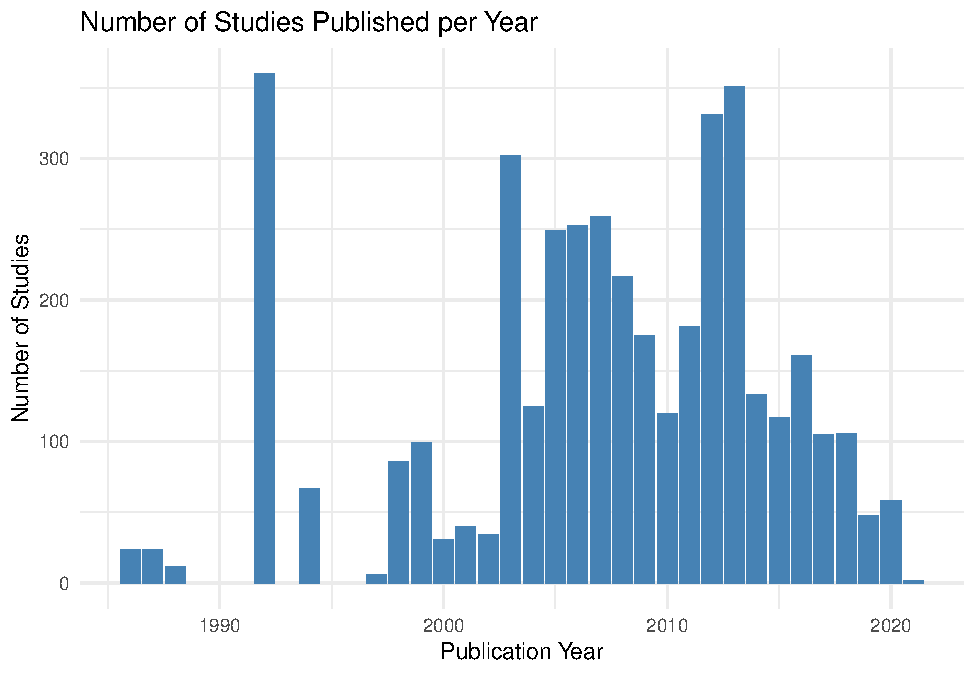
\includegraphics{_main_files/figure-latex/unnamed-chunk-5-1.pdf}

\subsection{Cumulative Sum Graph}\label{cumulative-sum-graph}

This graph displays the cumulative count of studies published over the years.
It helps visualize how the total number of studies increases as time progresses.

\begin{Shaded}
\begin{Highlighting}[]
\CommentTok{\# Cumulative Sum Graph}
\NormalTok{cumulative\_data }\OtherTok{\textless{}{-}}\NormalTok{ count\_data }\SpecialCharTok{\%\textgreater{}\%}
  \FunctionTok{arrange}\NormalTok{(Year) }\SpecialCharTok{\%\textgreater{}\%}  \CommentTok{\# Ensure data is sorted by year}
  \FunctionTok{mutate}\NormalTok{(}\AttributeTok{Cumulative =} \FunctionTok{cumsum}\NormalTok{(Count))  }\CommentTok{\# Calculate cumulative count}

\CommentTok{\# Plot the cumulative sum graph}
\FunctionTok{ggplot}\NormalTok{(cumulative\_data, }\FunctionTok{aes}\NormalTok{(}\AttributeTok{x =}\NormalTok{ Year, }\AttributeTok{y =}\NormalTok{ Cumulative)) }\SpecialCharTok{+}
  \FunctionTok{geom\_line}\NormalTok{(}\AttributeTok{size =} \DecValTok{1}\NormalTok{, }\AttributeTok{color =} \StringTok{"darkgreen"}\NormalTok{) }\SpecialCharTok{+}  \CommentTok{\# Create a line graph}
  \FunctionTok{labs}\NormalTok{(}\AttributeTok{title =} \StringTok{"Cumulative Count of Studies Published"}\NormalTok{,}
       \AttributeTok{x =} \StringTok{"Year"}\NormalTok{,}
       \AttributeTok{y =} \StringTok{"Cumulative Count of Studies"}\NormalTok{) }\SpecialCharTok{+}
  \FunctionTok{theme\_minimal}\NormalTok{()  }\CommentTok{\# Use a minimal theme for clarity}
\end{Highlighting}
\end{Shaded}

\begin{verbatim}
## Warning: Using `size` aesthetic for lines was deprecated in ggplot2 3.4.0.
## i Please use `linewidth` instead.
## This warning is displayed once every 8 hours.
## Call `lifecycle::last_lifecycle_warnings()` to see where this warning was
## generated.
\end{verbatim}

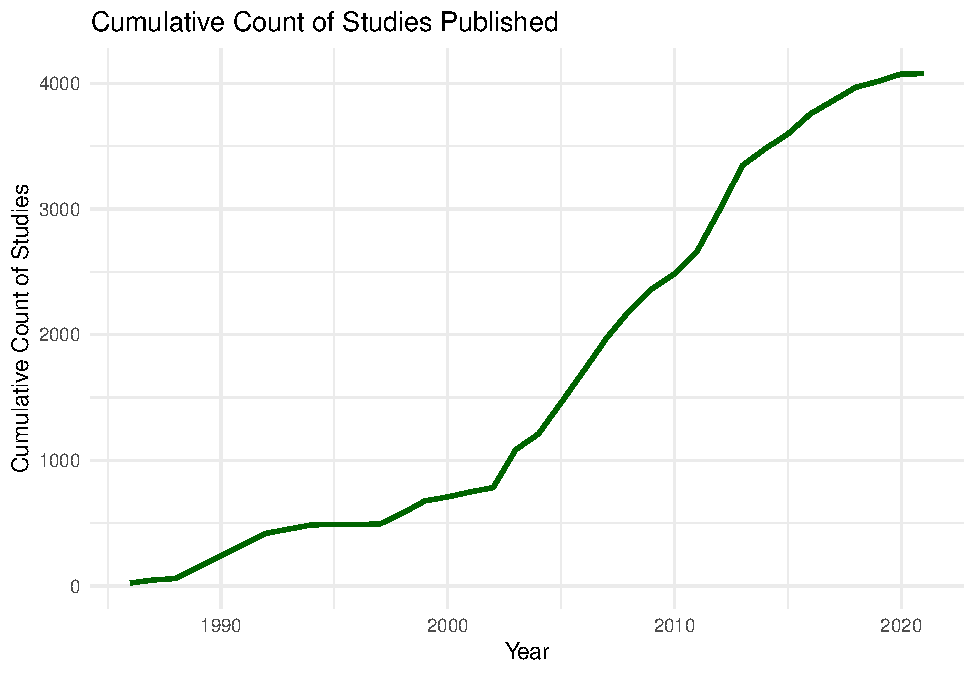
\includegraphics{_main_files/figure-latex/unnamed-chunk-6-1.pdf}

\subsection{Grouped Graph by categories}\label{grouped-graph-by-categories}

This graph shows the cumulative count of studies based on different crop types.
It allows for comparison of study trends across various crop systems.

\begin{Shaded}
\begin{Highlighting}[]
\CommentTok{\# Grouped Graph by Crop}
\NormalTok{grouped\_data }\OtherTok{\textless{}{-}}\NormalTok{ TAB }\SpecialCharTok{\%\textgreater{}\%}
 \FunctionTok{group\_by}\NormalTok{(Year, System\_C) }\SpecialCharTok{\%\textgreater{}\%} \FunctionTok{summarise}\NormalTok{(}\AttributeTok{Count =} \FunctionTok{n}\NormalTok{(),}\AttributeTok{.groups =} \StringTok{"drop"}\NormalTok{) }\SpecialCharTok{\%\textgreater{}\%}
  \FunctionTok{arrange}\NormalTok{(Year) }\SpecialCharTok{\%\textgreater{}\%}
  \FunctionTok{group\_by}\NormalTok{(System\_C) }\SpecialCharTok{\%\textgreater{}\%}
\FunctionTok{mutate}\NormalTok{(}\AttributeTok{Cumulative =} \FunctionTok{cumsum}\NormalTok{(Count)) }\SpecialCharTok{\%\textgreater{}\%} 
  \FunctionTok{ungroup}\NormalTok{()}

\CommentTok{\# Plot the grouped cumulative count graph}

\FunctionTok{ggplot}\NormalTok{(grouped\_data, }\FunctionTok{aes}\NormalTok{(}\AttributeTok{x =}\NormalTok{ Year, }\AttributeTok{y =}\NormalTok{ Cumulative, }\AttributeTok{color =}\NormalTok{ System\_C, }\AttributeTok{group =}\NormalTok{ System\_C)) }\SpecialCharTok{+}
  \FunctionTok{geom\_line}\NormalTok{(}\AttributeTok{size =} \DecValTok{1}\NormalTok{) }\SpecialCharTok{+} 
  \FunctionTok{geom\_point}\NormalTok{(}\AttributeTok{size =} \DecValTok{2}\NormalTok{) }\SpecialCharTok{+} 
  \FunctionTok{labs}\NormalTok{(}\AttributeTok{title =} \StringTok{"Cumulative Count of Studies per Control Type"}\NormalTok{, }
       \AttributeTok{x =} \StringTok{"Year"}\NormalTok{, }
       \AttributeTok{y =} \StringTok{"Cumulative Count of Studies"}\NormalTok{) }\SpecialCharTok{+}
  \FunctionTok{theme\_minimal}\NormalTok{()}
\end{Highlighting}
\end{Shaded}

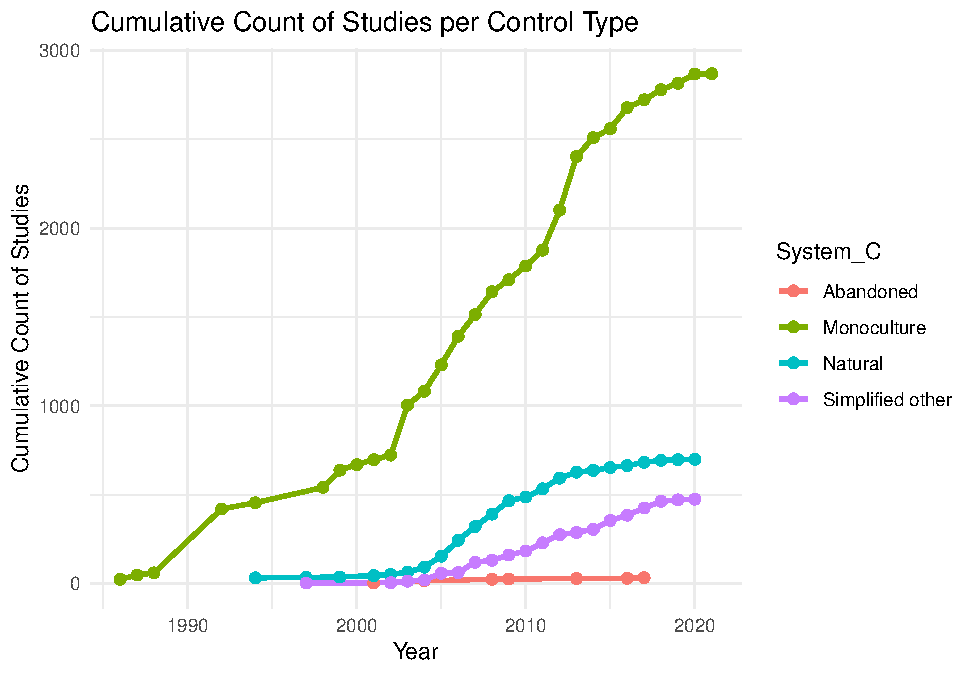
\includegraphics{_main_files/figure-latex/unnamed-chunk-7-1.pdf}

\section{Brief Note on Cumulative Meta-Analyses}\label{brief-note-on-cumulative-meta-analyses}

Cumulative meta-analyses are another important aspect of temporal analysis.
They allow researchers to assess how the effect sizes of interventions or phenomena change as new studies are added over time.
This approach can provide valuable insights into the robustness of findings and help track the evolution of evidence on specific topics.
Cumulative meta-analyses can further enrich evidence maps by providing a more nuanced understanding of how knowledge accumulates and shifts within a research domain.

By integrating temporal analysis into evidence maps and meta-analyses, researchers can enhance the depth and relevance of their findings, ultimately contributing to a more robust and informed understanding of research trends and their implications.

\chapter{Spatial Analyses and Exploration for Evidence Maps}\label{spatial-analyses-and-exploration-for-evidence-maps}

Spatial analysis is an invaluable tool for meta-analyses and evidence maps, enabling researchers to explore how intervention outcomes and environmental impacts vary across different geographic contexts.
In meta-analytic research, spatial dimensions often add a critical layer of understanding that cannot be captured through temporal or non-spatial methods alone.
For example, the geographic distribution of evidence can reveal clusters of research in certain regions or highlight underrepresented areas that might need targeted studies or interventions.
This spatial context becomes even more relevant when interventions are applied in fields such as agriculture or ecology, where environmental heterogeneity significantly influences intervention outcomes.

In meta-analyses, spatial data is often available in the form of GPS coordinates (point data), though precision can vary.
This variability poses challenges but also offers opportunities for spatial exploration at different scales.
Depending on the granularity and completeness of spatial data, researchers can choose from a range of spatial units for analysis, including administrative boundaries (e.g., country, region), environmental zones (e.g., biomes), or climate classifications.
By considering these spatial frameworks, it becomes possible to detect location-specific patterns, assess the transferability of interventions across ecological zones, and draw more nuanced conclusions that account for geographic variability.

Additionally, experimental data can be enriched by integrating geolocated climate or soil data from global or regional databases, such as WorldClim, TerraClimate, or the Harmonized World Soil Database.
These external datasets allow researchers to map experimental sites onto broader environmental gradients, thereby capturing key contextual factors like precipitation, temperature, or soil texture that might moderate intervention effects.
This comprehensive spatial integration provides a richer understanding of the environmental conditions underlying intervention success and helps refine location-specific recommendations

\subsection{Recommended Graph Types for Spatial Analysis}\label{recommended-graph-types-for-spatial-analysis}

\begin{enumerate}
\def\labelenumi{\arabic{enumi}.}
\item
  \textbf{Choropleth Maps}: Choropleth maps use different color intensities to represent the value of a variable across predefined spatial units (e.g., countries, regions, or districts).
  These maps are effective for visualizing spatial distributions of interventions or outcomes and can highlight regions of high or low research density.
\item
  \textbf{Whitaker Plots:} Whitaker plots are particularly useful for visualizing the distribution of study sites or intervention outcomes across ecological or climatic gradients, such as biomes or climate zones.
  This visualization technique is valuable in meta-analyses focusing on agroecological or environmental interventions, as it emphasizes the interaction between climatic conditions and intervention effectiveness.
  By illustrating how study outcomes vary across different ecological contexts, Whitaker plots enable researchers to identify key environmental factors that may influence the success of interventions, facilitating more tailored and effective recommendations.
\end{enumerate}

\subsection{Examples of Spatial Analysis in R}\label{examples-of-spatial-analysis-in-r}

For practical implementation, we recommend utilizing a suite of R packages that facilitate efficient spatial data handling and visualization, including \texttt{sf}, \texttt{sp}, \texttt{terra}, \texttt{raster}, and \texttt{ggplot2}.

The \texttt{sf} package (Pebesma, 2022a) is designed for representing and working with spatial vector data, such as points, polygons, and lines, along with their associated attributes.
It employs \textbf{sf} objects, which extend data frames to contain collections of simple features or spatial objects with potentially linked data.

The \texttt{terra} package (Hijmans, 2022) provides robust functions for creating, reading, manipulating, and writing both raster and vector data.
Raster data is particularly valuable for representing spatially continuous phenomena, as it divides the study area into a grid of equally sized cells or pixels, each assigned a value corresponding to the variable of interest.
Notably, \texttt{terra} is the latest and most powerful tool for raster analyses, offering enhanced functionality and improved performance for working with spatial data.

Furthermore, the \texttt{naturalearth} package streamlines access to country boundaries directly from the internet, thereby eliminating the need for manual downloads and ensuring users have the most current spatial data available.

When performing spatial analyses, it is crucial to ensure that all datasets are in the same coordinate projection before extracting values based on latitude and longitude.
Inconsistent projections can lead to inaccuracies in analysis, so careful attention to this detail is essential for reliable results.
Below, we present examples of spatial analyses using sample data on intervention outcomes across different regions.

\subsubsection{Example 1: Creating a Choropleth Map}\label{example-1-creating-a-choropleth-map}

This example demonstrates how to create a basic choropleth map using \texttt{ggplot2} and the \texttt{sf} package.
The dataset represents intervention effectiveness scores across different European regions.

\begin{Shaded}
\begin{Highlighting}[]
\CommentTok{\# Install necessary packages (uncomment to install if not already done)\}}
\CommentTok{\# install.packages("rnaturalearth")}
\CommentTok{\# install.packages("sf")}
\CommentTok{\# install.packages("dplyr")}
\CommentTok{\# install.packages("ggplot2")}

\CommentTok{\# Load required libraries for map creation and data manipulation}
\FunctionTok{library}\NormalTok{(rnaturalearth)  }\CommentTok{\# For world map data}
\FunctionTok{library}\NormalTok{(sf)             }\CommentTok{\# For spatial data handling}
\FunctionTok{library}\NormalTok{(dplyr)          }\CommentTok{\# For data manipulation}
\FunctionTok{library}\NormalTok{(ggplot2)        }\CommentTok{\# For visualization}

\CommentTok{\# Load the dataset from the chosen CSV file}
\NormalTok{DATA }\OtherTok{\textless{}{-}}\NormalTok{ Outcome }\SpecialCharTok{\%\textgreater{}\%}
  \FunctionTok{mutate}\NormalTok{(}\AttributeTok{Country =} \FunctionTok{factor}\NormalTok{(}\FunctionTok{tolower}\NormalTok{(Country))) }\SpecialCharTok{\%\textgreater{}\%}
  \FunctionTok{rename}\NormalTok{(}\AttributeTok{geounit =}\NormalTok{ Country) }\SpecialCharTok{\%\textgreater{}\%}
  \FunctionTok{group\_by}\NormalTok{(geounit) }\SpecialCharTok{\%\textgreater{}\%}
  \FunctionTok{count}\NormalTok{()}

\CommentTok{\# Load the world map with medium scale}
\NormalTok{world }\OtherTok{\textless{}{-}}\NormalTok{ rnaturalearth}\SpecialCharTok{::}\FunctionTok{ne\_countries}\NormalTok{(}\AttributeTok{scale =} \StringTok{"medium"}\NormalTok{, }\AttributeTok{returnclass =} \StringTok{"sf"}\NormalTok{) }\SpecialCharTok{\%\textgreater{}\%}
  \FunctionTok{mutate}\NormalTok{(}\AttributeTok{geounit =} \FunctionTok{tolower}\NormalTok{(geounit)) }\SpecialCharTok{\%\textgreater{}\%}
  \CommentTok{\# Rename certain countries for consistency}
  \FunctionTok{mutate}\NormalTok{(}\AttributeTok{geounit =} \FunctionTok{case\_when}\NormalTok{(}
\NormalTok{    geounit }\SpecialCharTok{==} \StringTok{"united kingdom"} \SpecialCharTok{\textasciitilde{}} \StringTok{"uk"}\NormalTok{,}
\NormalTok{    geounit }\SpecialCharTok{==} \StringTok{"united states of america"} \SpecialCharTok{\textasciitilde{}} \StringTok{"usa"}\NormalTok{,}
    \ConstantTok{TRUE} \SpecialCharTok{\textasciitilde{}}\NormalTok{ geounit}
\NormalTok{  ))}

\CommentTok{\# Merge the world map with the study count data}
\NormalTok{world2 }\OtherTok{\textless{}{-}} \FunctionTok{merge}\NormalTok{(world, DATA, }\AttributeTok{by =} \StringTok{"geounit"}\NormalTok{, }\AttributeTok{all =} \ConstantTok{TRUE}\NormalTok{) }\SpecialCharTok{\%\textgreater{}\%}
  \CommentTok{\# Create a discrete variable for legend representation}
  \FunctionTok{mutate}\NormalTok{(}\AttributeTok{cut\_n =} \FunctionTok{cut}\NormalTok{(n, }\AttributeTok{breaks =} \FunctionTok{c}\NormalTok{(}\DecValTok{0}\NormalTok{, }\DecValTok{10}\NormalTok{, }\DecValTok{40}\NormalTok{, }\DecValTok{80}\NormalTok{, }\DecValTok{500}\NormalTok{), }\AttributeTok{include.lowest =} \ConstantTok{TRUE}\NormalTok{))}

\CommentTok{\# Create the map visualizing the number of publications}
\NormalTok{map\_plot }\OtherTok{\textless{}{-}} \FunctionTok{ggplot}\NormalTok{(world2) }\SpecialCharTok{+}
  \FunctionTok{geom\_sf}\NormalTok{(}\FunctionTok{aes}\NormalTok{(}\AttributeTok{fill =}\NormalTok{ cut\_n), }\AttributeTok{size =} \FloatTok{0.2}\NormalTok{, }\AttributeTok{color =} \StringTok{"gray20"}\NormalTok{) }\SpecialCharTok{+}
  \FunctionTok{guides}\NormalTok{(}\AttributeTok{fill =} \FunctionTok{guide\_legend}\NormalTok{(}\AttributeTok{reverse =} \ConstantTok{TRUE}\NormalTok{)) }\SpecialCharTok{+}
  \FunctionTok{labs}\NormalTok{(}
    \AttributeTok{fill =} \StringTok{\textquotesingle{}Nombre d}\SpecialCharTok{\textbackslash{}\textquotesingle{}}\StringTok{expériences\textquotesingle{}}\NormalTok{,}
    \AttributeTok{title =} \StringTok{\textquotesingle{}Répartition des publications par pays\textquotesingle{}}\NormalTok{,}
    \AttributeTok{x =} \ConstantTok{NULL}\NormalTok{,}
    \AttributeTok{y =} \ConstantTok{NULL}
\NormalTok{  ) }\SpecialCharTok{+}
  \FunctionTok{theme\_classic}\NormalTok{() }\SpecialCharTok{+}
  \FunctionTok{scale\_fill\_manual}\NormalTok{(}\AttributeTok{values =} \FunctionTok{c}\NormalTok{(}\StringTok{\textquotesingle{}\#f6e8c3\textquotesingle{}}\NormalTok{, }\StringTok{"\#dfc283"}\NormalTok{, }\StringTok{\textquotesingle{}\#ba966c\textquotesingle{}}\NormalTok{, }\StringTok{\textquotesingle{}\#e5f5e0\textquotesingle{}}\NormalTok{, }\StringTok{\textquotesingle{}\#a1d99b\textquotesingle{}}\NormalTok{, }\StringTok{\textquotesingle{}\#31a354\textquotesingle{}}\NormalTok{), }\AttributeTok{na.value =} \StringTok{"white"}\NormalTok{)}

\CommentTok{\# Display the map}
\NormalTok{map\_plot}
\end{Highlighting}
\end{Shaded}

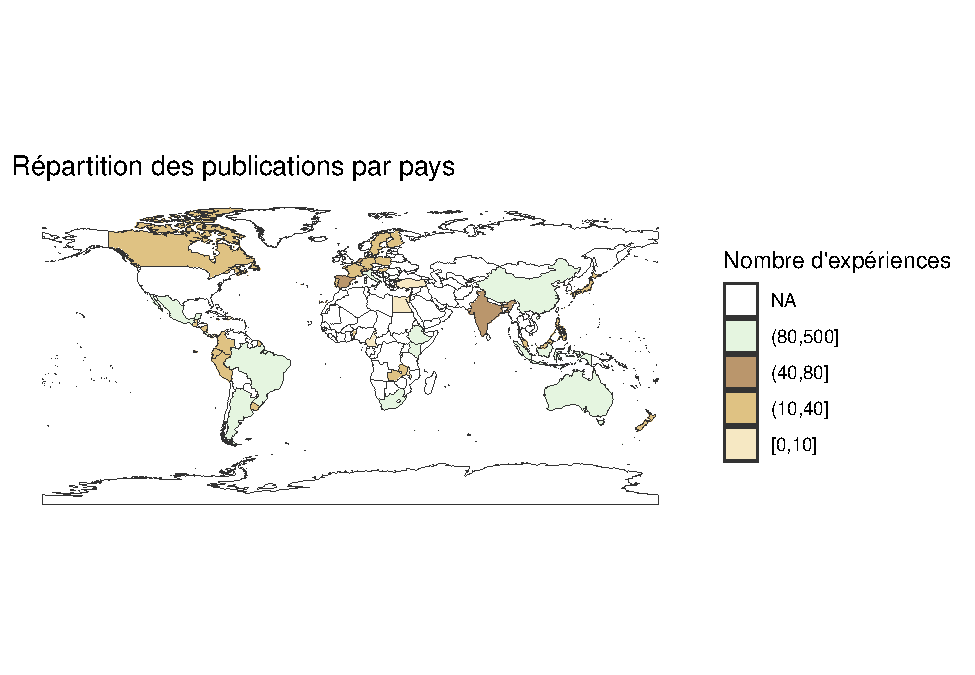
\includegraphics{_main_files/figure-latex/unnamed-chunk-8-1.pdf}

\subsection{Example 2: Creating a Whitaker Plot}\label{example-2-creating-a-whitaker-plot}

This example illustrates how to create a Whitaker plot using \texttt{ggplot2}.

\begin{Shaded}
\begin{Highlighting}[]
\CommentTok{\# Install the plotbiomes package from GitHub (uncomment to install if not done yet)}
\CommentTok{\# install.packages("devtools")}
\CommentTok{\# devtools::install\_github("valentinitnelav/plotbiomes")}

\CommentTok{\# Load necessary libraries}
\FunctionTok{library}\NormalTok{(plotbiomes)}
\FunctionTok{library}\NormalTok{(sp)}
\FunctionTok{library}\NormalTok{(raster)}
\FunctionTok{library}\NormalTok{(ggplot2)}

\CommentTok{\# Load temperature and precipitation raster data}
\NormalTok{path }\OtherTok{\textless{}{-}} \FunctionTok{system.file}\NormalTok{(}\StringTok{"extdata"}\NormalTok{, }\StringTok{"temp\_pp.tif"}\NormalTok{, }\AttributeTok{package =} \StringTok{"plotbiomes"}\NormalTok{)}
\NormalTok{temp\_pp }\OtherTok{\textless{}{-}}\NormalTok{ raster}\SpecialCharTok{::}\FunctionTok{stack}\NormalTok{(path)}
\FunctionTok{names}\NormalTok{(temp\_pp) }\OtherTok{\textless{}{-}} \FunctionTok{c}\NormalTok{(}\StringTok{"temperature"}\NormalTok{, }\StringTok{"precipitation"}\NormalTok{)}

\CommentTok{\# Prepare spatial coordinates from Outcome dataset}
\NormalTok{coordinates }\OtherTok{\textless{}{-}} \FunctionTok{cbind}\NormalTok{(}\FunctionTok{as.numeric}\NormalTok{(Outcome}\SpecialCharTok{$}\NormalTok{Lat\_C), }\FunctionTok{as.numeric}\NormalTok{(Outcome}\SpecialCharTok{$}\NormalTok{Lat\_T))}
\NormalTok{coordinates[}\FunctionTok{is.na}\NormalTok{(coordinates)] }\OtherTok{\textless{}{-}} \DecValTok{1}  \CommentTok{\# Handle NA values}
\NormalTok{spatial\_points }\OtherTok{\textless{}{-}} \FunctionTok{SpatialPoints}\NormalTok{(coordinates)}

\CommentTok{\# Extract temperature and precipitation values from the raster datasets}
\NormalTok{extractions }\OtherTok{\textless{}{-}}\NormalTok{ raster}\SpecialCharTok{::}\FunctionTok{extract}\NormalTok{(temp\_pp, spatial\_points, }\AttributeTok{df =} \ConstantTok{TRUE}\NormalTok{)}

\CommentTok{\# Adjust temperature values (WorldClim temperature data has a scale factor of 10)}
\NormalTok{extractions}\SpecialCharTok{$}\NormalTok{temperature }\OtherTok{\textless{}{-}}\NormalTok{ extractions}\SpecialCharTok{$}\NormalTok{temperature }\SpecialCharTok{/} \DecValTok{10}

\CommentTok{\# Convert precipitation from mm to cm}
\NormalTok{extractions}\SpecialCharTok{$}\NormalTok{precipitation }\OtherTok{\textless{}{-}}\NormalTok{ extractions}\SpecialCharTok{$}\NormalTok{precipitation }\SpecialCharTok{/} \DecValTok{10}

\CommentTok{\# Create a Whittaker base plot and add the temperature{-}precipitation data points}
\FunctionTok{whittaker\_base\_plot}\NormalTok{() }\SpecialCharTok{+}
  \FunctionTok{geom\_point}\NormalTok{(}\AttributeTok{data =}\NormalTok{ extractions, }
             \FunctionTok{aes}\NormalTok{(}\AttributeTok{x =}\NormalTok{ temperature, }
                 \AttributeTok{y =}\NormalTok{ precipitation), }
             \AttributeTok{size =} \DecValTok{3}\NormalTok{,}
             \AttributeTok{shape =} \DecValTok{21}\NormalTok{,}
             \AttributeTok{color =} \StringTok{"gray95"}\NormalTok{, }
             \AttributeTok{fill =} \StringTok{"black"}\NormalTok{,}
             \AttributeTok{stroke =} \DecValTok{1}\NormalTok{,}
             \AttributeTok{alpha =} \FloatTok{0.5}\NormalTok{) }\SpecialCharTok{+}
  \FunctionTok{theme\_bw}\NormalTok{() }\SpecialCharTok{+}
  \FunctionTok{labs}\NormalTok{(}
    \AttributeTok{title =} \StringTok{"Temperature vs. Precipitation"}\NormalTok{,}
    \AttributeTok{x =} \StringTok{"Temperature (°C)"}\NormalTok{,}
    \AttributeTok{y =} \StringTok{"Precipitation (cm)"}
\NormalTok{  )}
\end{Highlighting}
\end{Shaded}

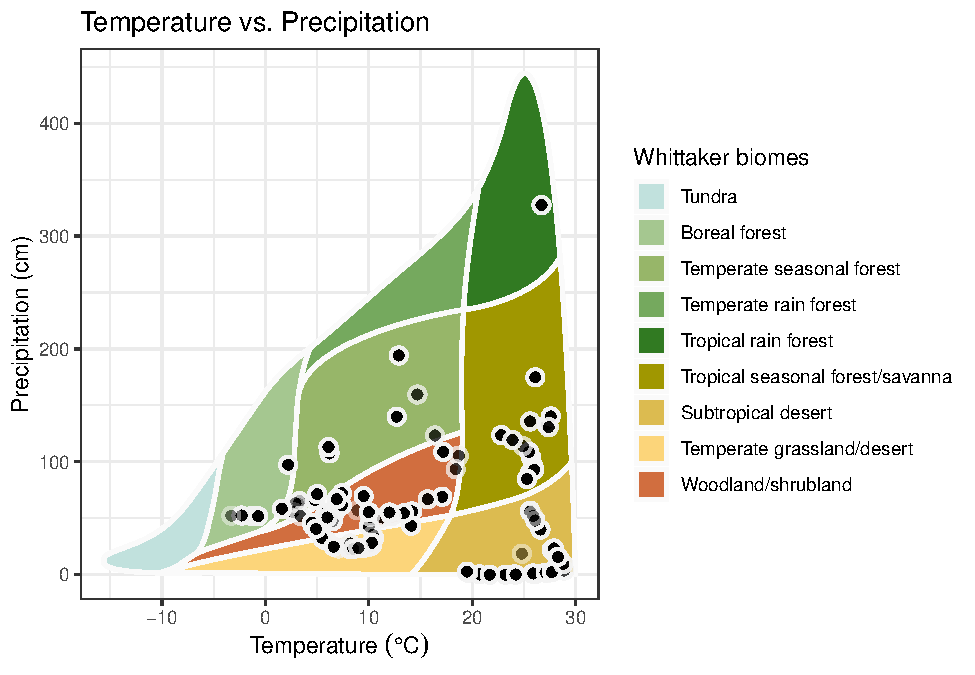
\includegraphics{_main_files/figure-latex/unnamed-chunk-9-1.pdf}

\chapter{2D Analyses for Meta-analyses and Evidence Maps}\label{d-analyses-for-meta-analyses-and-evidence-maps}

Two-dimensional (2-D) analyses are essential tools in meta-analyses and evidence maps, allowing researchers to explore relationships between variables, detect patterns, and effectively summarize complex data.
These techniques visualize interactions and distributions across two variables, providing a structured way to present findings.
From contingency tables that organize categorical data to heatmaps that reveal patterns of concentration, 2-D visualizations are highly versatile and can accommodate both qualitative and quantitative information.

This chapter presents key 2-D analytical techniques---including contingency tables, heatmaps, and interactive tables---that are particularly useful in meta-analytic contexts.
We will discuss when to use each approach, provide practical examples using R, and highlight their value for synthesizing and interpreting research evidence.

\section{Key 2-D Analysis Techniques}\label{key-2-d-analysis-techniques}

\begin{itemize}
\item
  Contingency Tables: Contingency tables, also known as cross-tabulations, summarize the distribution of two categorical variables in a matrix format.
  They display the frequency or proportion of observations that fall into each category combination, helping to identify relationships or dependencies between variables.
  Use Case: Useful for summarizing the types of interventions applied across different farm types or regions, or for examining the association between two categorical outcomes (e.g., intervention success vs.~failure across different management practices).
\item
  Heatmaps: Heatmaps use color gradients to represent the values of a variable within a 2-D space, making it easy to spot high and low concentrations.
  In meta-analysis, heatmaps can visually summarize study characteristics, intervention effects, or evidence distribution across multiple dimensions.
  Use Case: Ideal for visualizing the intensity of evidence coverage (e.g., number of studies by region and intervention type) or effect sizes across multiple subcategories.
\item
  Interactive Tables : Interactive tables enable researchers to explore data dynamically by sorting, filtering, and aggregating information directly within the table.
  Tools like DT in R or pivot tables in Excel provide flexibility for engaging with complex datasets, facilitating deeper exploration and comparison of study characteristics.
  Use Case: Effective for summarizing large evidence databases where users need to explore specific subsets (e.g., interventions, regions, outcomes) without losing track of the broader dataset.
\end{itemize}

\section{Practical Examples in R}\label{practical-examples-in-r}

To implement these 2-D analysis techniques in R, we recommend using packages such as tidyverse, tableone, gplots, and DT for creating contingency tables, heatmaps, and interactive tables.
Below, we illustrate how to construct and interpret each of these visualizations using sample data.

\subsection{Example 1: Creating a Simple Contingency Table}\label{example-1-creating-a-simple-contingency-table}

A contingency table helps summarize the frequency of two categorical variables.
In this example, we cross-tabulate intervention type and region to identify patterns in research distribution.

\begin{Shaded}
\begin{Highlighting}[]
\CommentTok{\# Load required libraries}
\FunctionTok{library}\NormalTok{(tidyverse)}

\NormalTok{contingency }\OtherTok{\textless{}{-}}\NormalTok{ Outcome }\SpecialCharTok{\%\textgreater{}\%} 
  \FunctionTok{group\_by}\NormalTok{(System\_C,System\_T) }\SpecialCharTok{\%\textgreater{}\%} 
  \FunctionTok{count}\NormalTok{()}

\CommentTok{\# Create contingency table}
\NormalTok{contingency\_table }\OtherTok{\textless{}{-}} \FunctionTok{table}\NormalTok{(Outcome}\SpecialCharTok{$}\NormalTok{Crop\_FAO\_C, Outcome}\SpecialCharTok{$}\NormalTok{System\_C)}

\CommentTok{\# Display as a data frame}
\FunctionTok{as.data.frame.matrix}\NormalTok{(contingency\_table)}
\end{Highlighting}
\end{Shaded}

\begin{verbatim}
##                                                     Abandoned Monoculture
## 1 - CEREALS AND CEREAL PRODUCTS                             0         841
## 10 - SPICES                                                 0           8
## 11 - FODDER CROPS AND PRODUCTS                              0          29
## 12 - STIMULANT CROPS AND DERIVED PRODUCTS                   0         194
## 2 - ROOTS AND TUBERS AND DERIVED PRODUCTS                   0          28
## 3 - SUGAR CROPS AND SWEETENERS AND DERIVED PRODUCTS         0           2
## 4 - PULSES AND DERIVED PRODUCTS                             0           4
## 5 - NUTS AND DERIVED PRODUCTS                               0          18
## 6 - OIL-BEARING CROPS AND DERIVED PRODUCTS                  0         222
## 7 - VEGETABLES AND DERIVED PRODUCTS                         0         560
## 8 - FRUITS AND DERIVED PRODUCTS                             0         588
## 9 - FIBRES OF VEGETAL AND ANIMAL ORIGIN                     0         305
## NA                                                         25           0
## Other or nd                                                 8          70
##                                                     Natural Simplified other
## 1 - CEREALS AND CEREAL PRODUCTS                           0               55
## 10 - SPICES                                               0                0
## 11 - FODDER CROPS AND PRODUCTS                           26               71
## 12 - STIMULANT CROPS AND DERIVED PRODUCTS                 0              194
## 2 - ROOTS AND TUBERS AND DERIVED PRODUCTS                 0                5
## 3 - SUGAR CROPS AND SWEETENERS AND DERIVED PRODUCTS       0                0
## 4 - PULSES AND DERIVED PRODUCTS                           0                0
## 5 - NUTS AND DERIVED PRODUCTS                             0                0
## 6 - OIL-BEARING CROPS AND DERIVED PRODUCTS                0               33
## 7 - VEGETABLES AND DERIVED PRODUCTS                       0               23
## 8 - FRUITS AND DERIVED PRODUCTS                           0               60
## 9 - FIBRES OF VEGETAL AND ANIMAL ORIGIN                   0                0
## NA                                                      673                0
## Other or nd                                               0               34
\end{verbatim}

\subsection{Example 2: Generating a Heatmap}\label{example-2-generating-a-heatmap}

Heatmaps are excellent for visualizing interactions or intensities.
This example uses a heatmap to display intervention effect sizes across different farm types.

\begin{Shaded}
\begin{Highlighting}[]
\CommentTok{\# Load required libraries}
\FunctionTok{library}\NormalTok{(ggplot2)}

\CommentTok{\# Create sample data}
\NormalTok{heatmap\_data }\OtherTok{\textless{}{-}}\NormalTok{ Outcome }\SpecialCharTok{\%\textgreater{}\%} 
  \FunctionTok{group\_by}\NormalTok{(System\_C,System\_T) }\SpecialCharTok{\%\textgreater{}\%} 
  \FunctionTok{count}\NormalTok{()}

\CommentTok{\# Create heatmap}
\FunctionTok{ggplot}\NormalTok{(heatmap\_data, }\FunctionTok{aes}\NormalTok{(}\AttributeTok{x =}\NormalTok{ System\_C, }\AttributeTok{y =}\NormalTok{ System\_T, }\AttributeTok{fill =}\NormalTok{ n)) }\SpecialCharTok{+}
  \FunctionTok{geom\_tile}\NormalTok{() }\SpecialCharTok{+}
  \FunctionTok{scale\_fill\_gradient2}\NormalTok{(}\AttributeTok{low =} \StringTok{"red"}\NormalTok{, }\AttributeTok{high =} \StringTok{"blue"}\NormalTok{, }\AttributeTok{mid =} \StringTok{"white"}\NormalTok{, }\AttributeTok{midpoint =} \DecValTok{0}\NormalTok{) }\SpecialCharTok{+}
  \FunctionTok{theme\_minimal}\NormalTok{() }\SpecialCharTok{+}
  \FunctionTok{labs}\NormalTok{(}\AttributeTok{title =} \StringTok{"Number of studies far various control X treatment combination"}\NormalTok{,}
       \AttributeTok{fill =} \StringTok{"Number of studies"}\NormalTok{)}
\end{Highlighting}
\end{Shaded}

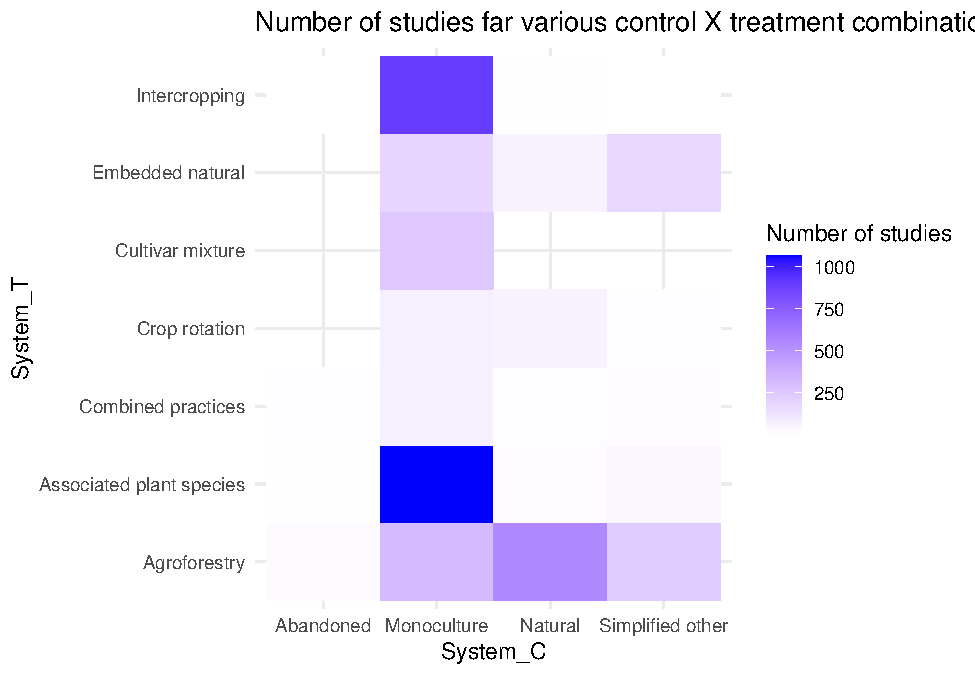
\includegraphics{_main_files/figure-latex/unnamed-chunk-11-1.pdf}

\subsection{Example 3: Bubble plots}\label{example-3-bubble-plots}

Bubble plots are useful for showing interactions between different categories and the size of intervention effects.
They encode information through the position, size, and color of the bubbles, making it easy to see patterns and differences.
For example, a bubble plot can show intervention effects across various farm types, with larger bubbles indicating stronger effects.
This helps highlight which interventions work best in different contexts.

\begin{Shaded}
\begin{Highlighting}[]
\CommentTok{\# Load required libraries}
\FunctionTok{library}\NormalTok{(ggplot2)}

\CommentTok{\# Create sample data}
\NormalTok{bubble\_data }\OtherTok{\textless{}{-}}\NormalTok{ Outcome }\SpecialCharTok{\%\textgreater{}\%} 
  \FunctionTok{group\_by}\NormalTok{(System\_C,System\_T) }\SpecialCharTok{\%\textgreater{}\%} 
  \FunctionTok{count}\NormalTok{()}

\CommentTok{\# Créez un graphique à bulles}
\NormalTok{bubble\_plot }\OtherTok{\textless{}{-}} \FunctionTok{ggplot}\NormalTok{(bubble\_data, }\FunctionTok{aes}\NormalTok{(}\AttributeTok{x =}\NormalTok{ System\_C, }\AttributeTok{y =}\NormalTok{ System\_T)) }\SpecialCharTok{+}
  \FunctionTok{geom\_point}\NormalTok{(}\FunctionTok{aes}\NormalTok{(}\AttributeTok{size =}\NormalTok{ n, }\AttributeTok{fill =}\NormalTok{ n, }\AttributeTok{color =}\NormalTok{ n), }\AttributeTok{alpha =} \FloatTok{0.75}\NormalTok{, }\AttributeTok{shape =} \DecValTok{21}\NormalTok{) }\SpecialCharTok{+} 
  \CommentTok{\# Échelle personnalisée pour la taille des bulles}
  \FunctionTok{scale\_size\_continuous}\NormalTok{(}
    \AttributeTok{limits =} \FunctionTok{c}\NormalTok{(}\FloatTok{0.000001}\NormalTok{, }\DecValTok{100}\NormalTok{),  }\CommentTok{\# Limites personnalisées}
    \AttributeTok{range =} \FunctionTok{c}\NormalTok{(}\DecValTok{3}\NormalTok{, }\DecValTok{15}\NormalTok{),           }\CommentTok{\# Plage de tailles personnalisées}
    \AttributeTok{breaks =} \FunctionTok{c}\NormalTok{(}\DecValTok{1}\NormalTok{, }\DecValTok{10}\NormalTok{, }\DecValTok{50}\NormalTok{, }\DecValTok{75}\NormalTok{),  }\CommentTok{\# Points de rupture pour les étiquettes de taille}
    \AttributeTok{labels =} \FunctionTok{c}\NormalTok{(}\StringTok{"1\%"}\NormalTok{, }\StringTok{"10\%"}\NormalTok{, }\StringTok{"50\%"}\NormalTok{, }\StringTok{"75\%"}\NormalTok{)  }\CommentTok{\# Étiquettes pour les tailles}
\NormalTok{  ) }\SpecialCharTok{+} 
  \CommentTok{\# Personnalisez les légendes}
  \FunctionTok{labs}\NormalTok{(}
    \AttributeTok{x =} \StringTok{""}\NormalTok{,}
    \AttributeTok{y =} \StringTok{""}\NormalTok{,}
    \AttributeTok{size =} \StringTok{"Abondance relative (\%)"}\NormalTok{,}
    \AttributeTok{fill =} \StringTok{"Valeur"}\NormalTok{,}
    \AttributeTok{color =} \StringTok{"Valeur"}
\NormalTok{  ) }\SpecialCharTok{+} 
  \CommentTok{\# Personnalisez les thèmes pour une meilleure lisibilité}
  \FunctionTok{theme\_minimal}\NormalTok{() }\SpecialCharTok{+}
  \CommentTok{\# Personnalisez la palette de couleurs}
  \FunctionTok{scale\_fill\_gradient}\NormalTok{(}\AttributeTok{low =} \StringTok{"\#F1EEF6"}\NormalTok{, }\AttributeTok{high =} \StringTok{"\#54278F"}\NormalTok{) }\SpecialCharTok{+}
  \FunctionTok{scale\_color\_gradient}\NormalTok{(}\AttributeTok{low =} \StringTok{"\#F1EEF6"}\NormalTok{, }\AttributeTok{high =} \StringTok{"\#54278F"}\NormalTok{)}

\NormalTok{bubble\_plot}
\end{Highlighting}
\end{Shaded}

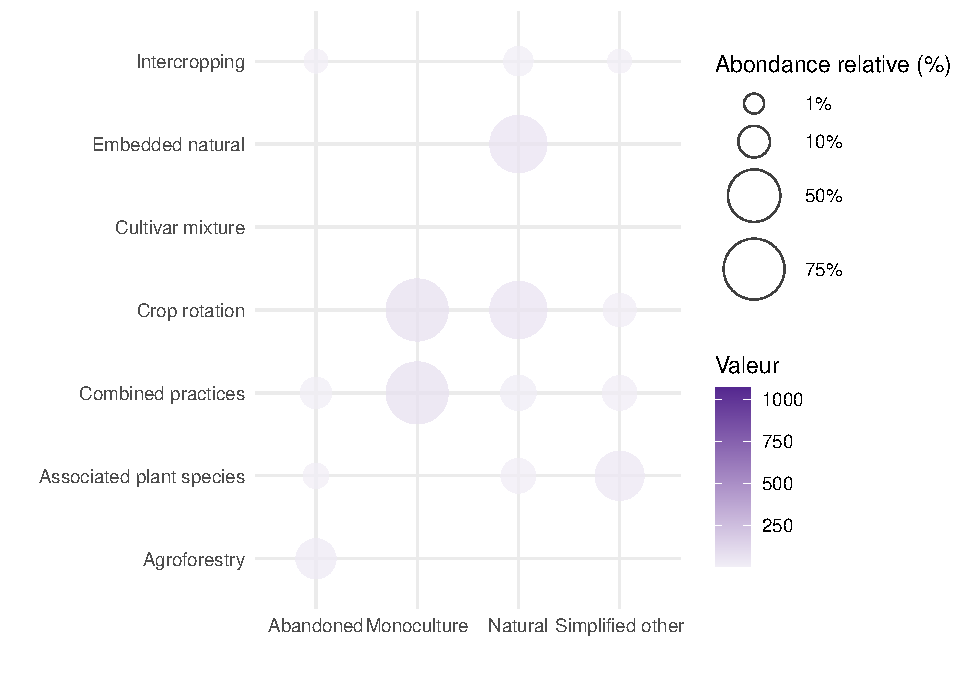
\includegraphics{_main_files/figure-latex/unnamed-chunk-12-1.pdf}

\subsection{Example 3: Building an Interactive Table}\label{example-3-building-an-interactive-table}

Interactive tables are useful for large datasets that require filtering or detailed inspection.
The \texttt{DT} package in R makes it easy to create tables that users can sort, search, and explore.

\begin{Shaded}
\begin{Highlighting}[]
\FunctionTok{library}\NormalTok{(reactable)}
\FunctionTok{library}\NormalTok{(dplyr)}
\FunctionTok{library}\NormalTok{(webshot)}

\CommentTok{\# Create a summary of grouped data}
\NormalTok{GROUP }\OtherTok{\textless{}{-}}\NormalTok{ Outcome }\SpecialCharTok{\%\textgreater{}\%}
  \FunctionTok{group\_by}\NormalTok{(System\_C) }\SpecialCharTok{\%\textgreater{}\%}
  \FunctionTok{summarize}\NormalTok{(}\AttributeTok{Number =} \FunctionTok{n}\NormalTok{(), }\AttributeTok{.groups =} \StringTok{"drop"}\NormalTok{)}


\NormalTok{react}\OtherTok{\textless{}{-}}\FunctionTok{reactable}\NormalTok{(}
\NormalTok{  GROUP,}
  \AttributeTok{details =} \ControlFlowTok{function}\NormalTok{(index) \{}
    \CommentTok{\# Filter the details for the selected group}
\NormalTok{    details\_data }\OtherTok{\textless{}{-}} \FunctionTok{filter}\NormalTok{(Outcome, System\_C }\SpecialCharTok{==}\NormalTok{ GROUP}\SpecialCharTok{$}\NormalTok{System\_C[index])}
    
    \CommentTok{\# Create a reactable for the detailed view}
\NormalTok{    tbl }\OtherTok{\textless{}{-}} \FunctionTok{reactable}\NormalTok{(details\_data,}
          \AttributeTok{columns =} \FunctionTok{list}\NormalTok{(}
  \AttributeTok{System\_C =} \FunctionTok{colDef}\NormalTok{(}
    \AttributeTok{style =} \ControlFlowTok{function}\NormalTok{(value) \{}
      \ControlFlowTok{if}\NormalTok{ (value }\SpecialCharTok{\textgreater{}} \DecValTok{0}\NormalTok{) \{}
\NormalTok{        color }\OtherTok{\textless{}{-}} \StringTok{"\#008000"}
\NormalTok{      \} }\ControlFlowTok{else} \ControlFlowTok{if}\NormalTok{ (value }\SpecialCharTok{\textless{}} \DecValTok{0}\NormalTok{) \{}
\NormalTok{        color }\OtherTok{\textless{}{-}} \StringTok{"\#e00000"}
\NormalTok{      \} }\ControlFlowTok{else}\NormalTok{ \{}
\NormalTok{        color }\OtherTok{\textless{}{-}} \StringTok{"\#777"}
\NormalTok{      \}}
      \FunctionTok{list}\NormalTok{(}\AttributeTok{color =}\NormalTok{ color, }\AttributeTok{fontWeight =} \StringTok{"bold"}\NormalTok{)}
\NormalTok{    \}}
\NormalTok{  )}
\NormalTok{))}
\NormalTok{    htmltools}\SpecialCharTok{::}\FunctionTok{div}\NormalTok{(}\AttributeTok{style =} \FunctionTok{list}\NormalTok{(}\AttributeTok{margin =} \StringTok{"12px 45px"}\NormalTok{), tbl)}
\NormalTok{  \},}
  \AttributeTok{onClick =} \StringTok{"expand"}\NormalTok{,  }\CommentTok{\# Set click behavior to expand row details}
  \AttributeTok{rowStyle =} \FunctionTok{list}\NormalTok{(}\AttributeTok{cursor =} \StringTok{"pointer"}\NormalTok{)  }\CommentTok{\# Change cursor style to pointer for rows}
\NormalTok{)}

\CommentTok{\#react}
\end{Highlighting}
\end{Shaded}


  \bibliography{book.bib,packages.bib}

\end{document}
